\documentclass[10pt,a4paper]{article}
\usepackage[margin=2cm]{geometry}
\usepackage{amsmath,amssymb,booktabs,tikz,hyperref,microtype}
\usetikzlibrary{arrows.meta,positioning}
\hypersetup{colorlinks,linkcolor=blue!50!black,urlcolor=blue!50!black}
\setlength{\parskip}{4pt}\setlength{\parindent}{0pt}
\title{\vspace{-1.2cm}FlyRunner: does a fly connectome help an agent play an endless runner?}
\author{Project write-up, September 2026}
\date{}

\begin{document}\maketitle\vspace{-0.9cm}

\section*{The question}
A connectome is a wiring diagram: which neurons connect to which, with how many synapses, and (where predicted)
whether the connection excites or inhibits. It has no trained weights and no dynamics. We took a task-relevant piece
of the \emph{Drosophila} male CNS connectome (MaleCNS v1.0), froze a neural network's wiring to it, left only a few
biologically unknown parameters free, and asked two things: can it be trained to play a 3-lane endless runner, and
does the \emph{real} wiring do better than a random wiring of the same size? Nothing here is a claim about how a
fly thinks.

\section*{How it works}
\begin{center}
\resizebox{\textwidth}{!}{%
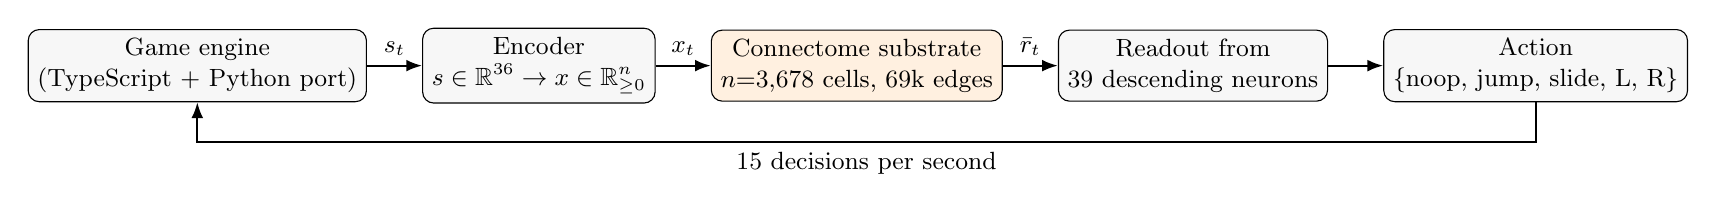
\begin{tikzpicture}[node distance=5mm and 7mm, every node/.style={font=\small},
  box/.style={draw, rounded corners, minimum height=8mm, minimum width=19mm, align=center, fill=gray!6},
  arr/.style={-{Latex[length=2mm]}, thick}]
\node[box] (game) {Game engine\\(TypeScript + Python port)};
\node[box, right=of game] (enc) {Encoder\\$s\in\mathbb{R}^{36}\to x\in\mathbb{R}^{n}_{\ge0}$};
\node[box, right=of enc, fill=orange!12] (sub) {Connectome substrate\\$n{=}3{,}678$ cells, 69k edges};
\node[box, right=of sub] (ro) {Readout from\\39 descending neurons};
\node[box, right=of ro] (act) {Action\\\{noop, jump, slide, L, R\}};
\draw[arr] (game) -- node[above]{$s_t$} (enc);
\draw[arr] (enc) -- node[above]{$x_t$} (sub);
\draw[arr] (sub) -- node[above]{$\bar r_t$} (ro);
\draw[arr] (ro) -- (act);
\draw[arr] (act.south) |- ++(0,-5mm) -| node[below, pos=0.25]{15 decisions per second} (game.south);
\end{tikzpicture}}
\end{center}

\textbf{The game.} An original three-lane runner with three kinds of obstacle: a log (jump), a beam (slide) and a
wall (change lane). The engine is small and deterministic, and exposes the four actions, a \texttt{step()}, and a
36-number state: which lane you are in, whether you are mid-jump or mid-slide, your speed, and for each lane the
type and distance of the next two obstacles. It was ported line for line to Python so that training runs fast,
and the port is checked against recorded trajectories from the original.

\textbf{The connectome piece.} From the public MaleCNS v1.0 data we keep the cell types a fly would use for this
task: the early visual system (photoreceptors, lamina, medulla, the T4/T5 motion detectors), the looming
detectors (LC4, LPLC2 and relatives), the pathway from the eye into the central complex (MeTu, TuBu, ring
neurons), the central complex itself (compass and steering cells), and 20 types of descending neuron (DN) that
carry commands to the body. We keep connections with at least 5 synapses, restrict the eye to a patch of 37
columns, drop any cell that is not on a path from input to a DN, and assign each connection a sign from its
predicted neurotransmitter. Result: 3{,}678 neurons and 69{,}127 connections. An early build had accidentally cut
the central complex off from the eye; the data itself showed which pathway was missing, and it was added.

\textbf{The network.} Each neuron is a leaky rate unit (the flyvis form of Lappalainen et al.\ 2024):
\begin{equation}
\tau_i\,\frac{dV_i}{dt} = -V_i + b_i + \sum_j W_{ij}\,r_j + g\,x_i,\qquad r_j=\max(V_j,0),\qquad
W_{ij} = \sigma_j\,\bigl|\alpha_{c(j,i)}\bigr|\,\frac{N_{ij}}{S}.
\end{equation}
Everything about the wiring is fixed: which pairs $(i,j)$ are connected, the synapse count $N_{ij}$, and the sign
$\sigma_j$ ($+1$ excitatory, $-1$ inhibitory). What can be learned is a time constant $\tau$ and bias $b$ per cell
type, and one scale $\alpha_c$ per class of connection $c$ (pre-type $\to$ post-type). No connection is ever
added and no sign can flip. $S$ just normalises synapse counts. The network is integrated in 10\,ms steps, seven
per decision. The encoder maps the game state onto the photoreceptor and lamina cells; the readout standardises the
39 DN activities and passes them through a small $39{\to}32{\to}5$ layer to pick an action. Before training, a sweep
over the input gain $g$ and the initial scale finds a setting where the network is neither silent nor exploding.

\textbf{Controls.} To ask whether the real wiring matters we build, with the same code, a \emph{shuffled} graph
(same in- and out-degree for every cell, connections rewired) and a \emph{random} graph (same number of cells and
connections), and train each exactly the same way.

\section*{Training}
The reward per decision is metres advanced, plus 5 per coin, minus 50 for a crash. Episodes end at 180\,s.
A standard PPO learner (clipped objective, GAE with $\gamma{=}0.99$, $\lambda{=}0.95$) trains both a plain
$2{\times}64$ MLP baseline and the connectome agent, the latter with gradients passed back through the network's
dynamics over 32-decision windows:
\begin{equation}
L = \mathbb{E}_t\Bigl[\min\bigl(\rho_t\hat A_t,\ \mathrm{clip}(\rho_t,1{-}\epsilon,1{+}\epsilon)\hat A_t\bigr)\Bigr]
- c_v\,\mathbb{E}_t\bigl[(V_\theta(s_t)-\hat R_t)^2\bigr] + c_H\,\mathbb{E}_t\bigl[\mathcal H(\pi_\theta(\cdot|s_t))\bigr],
\qquad \rho_t=\frac{\pi_\theta(a_t|s_t)}{\pi_{\theta_{\text{old}}}(a_t|s_t)}.
\end{equation}
The first runs learned almost nothing. The reason turned out to be the game, not the learner: a good player
does nothing 96\% of the time, and a random \texttt{slide} while airborne cancels a jump. Under random
exploration a correct jump is undone with probability $1-0.8^{8}\approx0.83$, so the learner never gets credit
for it. Starting the policy with a strong bias towards ``do nothing'' fixed this; the MLP then reached the level
of a hand-written heuristic in about an hour.

The connectome agent, however, never got off the ground with PPO. So we tried imitation instead: train the
connectome agent to copy the MLP's decisions. Plain imitation copies the teacher on the teacher's own paths but
falls apart as soon as the student drifts off them, so we used DAgger, which repeatedly collects the states the
\emph{student} visits, labels them with the teacher, and retrains:
\begin{equation}
\mathcal D \leftarrow \mathcal D \cup \{(s, \pi^{*}(s)) : s \sim \pi_{\beta}\},\qquad
\pi_\beta = \beta\,\pi^{*} + (1-\beta)\,\hat\pi,\qquad
\hat\pi \leftarrow \operatorname*{arg\,min}_{\pi'}\ \mathbb{E}_{(s,a)\sim\mathcal D}\bigl[-\log\pi'(a|s)\bigr].
\end{equation}

\section*{Results}
Every agent is scored the same way: 200 unseen courses, 180\,s each (3{,}409\,m if you survive to the end).
\begin{center}\small
\begin{tabular}{@{}llrrr@{}}\toprule
agent & training & mean (m) & median & reached the end \\\midrule
random play & -- & 36 & 28 & 0\% \\
hand-written heuristic & -- & 1{,}209 & 952 & 1\% \\
MLP baseline, PPO & 75 min & 1{,}954 & 2{,}579 & 47\% \\\midrule
connectome, PPO from scratch & 45 min & 37 & 29 & 0\% \\
connectome, imitation only & 100 min & 111 & 91 & 0\% \\
connectome, imitation + DAgger & 8 h & \textbf{317} & 218 & 0\% \\\midrule
\multicolumn{5}{@{}l}{\emph{Same DAgger recipe from scratch, 6 h each, run side by side:}}\\
real wiring & & 188 & 164 & 0\% \\
shuffled wiring & & \textbf{423} & 306 & 0\% \\
random wiring & & \textbf{465} & 319 & 0\% \\\bottomrule
\end{tabular}
\end{center}

Three things came out of this. First, the connectome-constrained network \emph{can} be trained to play: 317\,m,
nine times random play, still improving when we stopped, and visibly dodging obstacles in the live demo. Second,
it is far behind the unconstrained MLP, because the wiring is fixed and only a few hundred numbers can change.
Third --- the main finding --- \textbf{the real wiring does not help}. Given the same training, a shuffled or
random graph of the same size learns two to two-and-a-half times better. The fly's eye-to-command pathway is deep
and dominated by inhibition, and turns out to be a harder thing to read a policy out of than a random graph, which
behaves like a well-mixed reservoir. This matches the caveat of the closest earlier project (Fly Dino: the circuit
is used, but there is no evidence the biology is what makes it work) and adds the control experiment that neither
it nor doomfly ran.

\textbf{Caveats.} One training run per condition, a few hours each on a laptop. Two changes could alter the
ranking and are the obvious next steps: letting every synapse have its own weight (rather than one per connection
class), and feeding the network rendered pixels instead of the game's state vector.

\textbf{Implementation.} \texttt{game/} is TypeScript (engine, three.js renderer, and a browser runtime that runs
exported agents directly, with a live panel showing activity by cell type). \texttt{flybrain/} is Python (data
pipeline, network, PPO, DAgger, evaluation, export). Everything is rebuilt from the public data with a manifest.
MaleCNS v1.0 is CC BY 4.0 (FlyEM/HHMI Janelia, University of Cambridge, MRC LMB, Google Research). This is an
independent project, not affiliated with the connectome or flyvis authors or any game studio.
\end{document}
